% fig_design.tex -- generated by gen_fig_design.py; do not edit by hand.
\definecolor{fpV}{HTML}{D55E00}\definecolor{fpB}{HTML}{0072B2}%
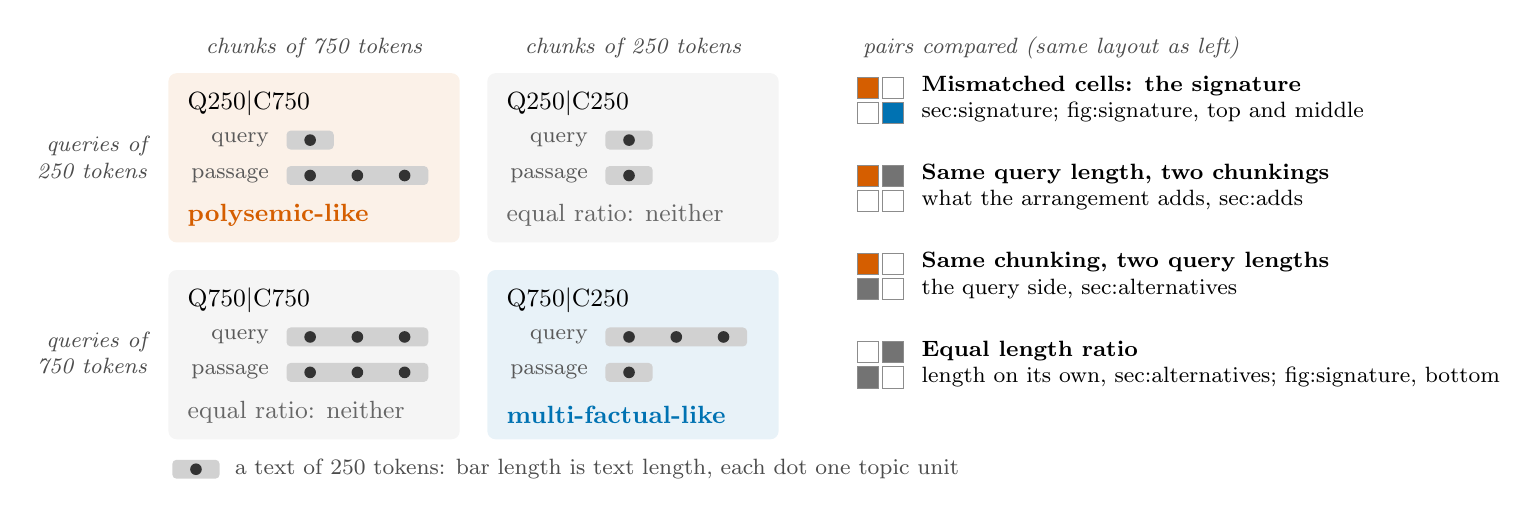
\begin{tikzpicture}[font=\small]
\fill[fpV!9, rounded corners=3pt] (0.00,0.00) rectangle (3.70,-2.15);
\node[anchor=north west, font=\small] at (0.12,-0.10) {Q250$|$C750};
\node[anchor=east, font=\footnotesize, black!65] at (1.40,-0.85) {query};
\fill[black!18, rounded corners=1.5pt] (1.50,-0.97) rectangle (2.10,-0.73);
\fill[black!80] (1.80,-0.85) circle (2.1pt);
\node[anchor=east, font=\footnotesize, black!65] at (1.40,-1.30) {passage};
\fill[black!18, rounded corners=1.5pt] (1.50,-1.42) rectangle (3.30,-1.18);
\fill[black!80] (1.80,-1.30) circle (2.1pt);
\fill[black!80] (2.40,-1.30) circle (2.1pt);
\fill[black!80] (3.00,-1.30) circle (2.1pt);
\node[anchor=south west, font=\small\bfseries, fpV] at (0.12,-2.07) {polysemic-like};
\fill[black!4, rounded corners=3pt] (4.05,0.00) rectangle (7.75,-2.15);
\node[anchor=north west, font=\small] at (4.17,-0.10) {Q250$|$C250};
\node[anchor=east, font=\footnotesize, black!65] at (5.45,-0.85) {query};
\fill[black!18, rounded corners=1.5pt] (5.55,-0.97) rectangle (6.15,-0.73);
\fill[black!80] (5.85,-0.85) circle (2.1pt);
\node[anchor=east, font=\footnotesize, black!65] at (5.45,-1.30) {passage};
\fill[black!18, rounded corners=1.5pt] (5.55,-1.42) rectangle (6.15,-1.18);
\fill[black!80] (5.85,-1.30) circle (2.1pt);
\node[anchor=south west, font=\small, black!60] at (4.17,-2.07) {equal ratio: neither};
\fill[black!4, rounded corners=3pt] (0.00,-2.50) rectangle (3.70,-4.65);
\node[anchor=north west, font=\small] at (0.12,-2.60) {Q750$|$C750};
\node[anchor=east, font=\footnotesize, black!65] at (1.40,-3.35) {query};
\fill[black!18, rounded corners=1.5pt] (1.50,-3.47) rectangle (3.30,-3.23);
\fill[black!80] (1.80,-3.35) circle (2.1pt);
\fill[black!80] (2.40,-3.35) circle (2.1pt);
\fill[black!80] (3.00,-3.35) circle (2.1pt);
\node[anchor=east, font=\footnotesize, black!65] at (1.40,-3.80) {passage};
\fill[black!18, rounded corners=1.5pt] (1.50,-3.92) rectangle (3.30,-3.68);
\fill[black!80] (1.80,-3.80) circle (2.1pt);
\fill[black!80] (2.40,-3.80) circle (2.1pt);
\fill[black!80] (3.00,-3.80) circle (2.1pt);
\node[anchor=south west, font=\small, black!60] at (0.12,-4.57) {equal ratio: neither};
\fill[fpB!9, rounded corners=3pt] (4.05,-2.50) rectangle (7.75,-4.65);
\node[anchor=north west, font=\small] at (4.17,-2.60) {Q750$|$C250};
\node[anchor=east, font=\footnotesize, black!65] at (5.45,-3.35) {query};
\fill[black!18, rounded corners=1.5pt] (5.55,-3.47) rectangle (7.35,-3.23);
\fill[black!80] (5.85,-3.35) circle (2.1pt);
\fill[black!80] (6.45,-3.35) circle (2.1pt);
\fill[black!80] (7.05,-3.35) circle (2.1pt);
\node[anchor=east, font=\footnotesize, black!65] at (5.45,-3.80) {passage};
\fill[black!18, rounded corners=1.5pt] (5.55,-3.92) rectangle (6.15,-3.68);
\fill[black!80] (5.85,-3.80) circle (2.1pt);
\node[anchor=south west, font=\small\bfseries, fpB] at (4.17,-4.57) {multi-factual-like};
\node[font=\footnotesize\itshape, black!70] at (1.85,0.32) {chunks of 750 tokens};
\node[font=\footnotesize\itshape, black!70] at (5.90,0.32) {chunks of 250 tokens};
\node[font=\footnotesize\itshape, black!70, anchor=east, align=right] at (-0.15,-1.07) {queries of\\250 tokens};
\node[font=\footnotesize\itshape, black!70, anchor=east, align=right] at (-0.15,-3.58) {queries of\\750 tokens};
\node[anchor=west, font=\footnotesize\itshape, black!70] at (8.70,0.32) {pairs compared (same layout as left)};
\filldraw[fill=fpV, draw=black!45, line width=0.4pt] (8.75,-0.05) rectangle (9.02,-0.32);
\filldraw[fill=white, draw=black!45, line width=0.4pt] (9.07,-0.05) rectangle (9.34,-0.32);
\filldraw[fill=white, draw=black!45, line width=0.4pt] (8.75,-0.37) rectangle (9.02,-0.64);
\filldraw[fill=fpB, draw=black!45, line width=0.4pt] (9.07,-0.37) rectangle (9.34,-0.64);
\node[anchor=north west, align=left, font=\footnotesize, inner sep=0pt] at (9.56,-0.03) {\textbf{Mismatched cells: the signature}\\\cref{sec:signature}; \cref{fig:signature}, top and middle};
\filldraw[fill=fpV, draw=black!45, line width=0.4pt] (8.75,-1.17) rectangle (9.02,-1.44);
\filldraw[fill=black!55, draw=black!45, line width=0.4pt] (9.07,-1.17) rectangle (9.34,-1.44);
\filldraw[fill=white, draw=black!45, line width=0.4pt] (8.75,-1.49) rectangle (9.02,-1.76);
\filldraw[fill=white, draw=black!45, line width=0.4pt] (9.07,-1.49) rectangle (9.34,-1.76);
\node[anchor=north west, align=left, font=\footnotesize, inner sep=0pt] at (9.56,-1.15) {\textbf{Same query length, two chunkings}\\what the arrangement adds, \cref{sec:adds}};
\filldraw[fill=fpV, draw=black!45, line width=0.4pt] (8.75,-2.29) rectangle (9.02,-2.56);
\filldraw[fill=white, draw=black!45, line width=0.4pt] (9.07,-2.29) rectangle (9.34,-2.56);
\filldraw[fill=black!55, draw=black!45, line width=0.4pt] (8.75,-2.61) rectangle (9.02,-2.88);
\filldraw[fill=white, draw=black!45, line width=0.4pt] (9.07,-2.61) rectangle (9.34,-2.88);
\node[anchor=north west, align=left, font=\footnotesize, inner sep=0pt] at (9.56,-2.27) {\textbf{Same chunking, two query lengths}\\the query side, \cref{sec:alternatives}};
\filldraw[fill=white, draw=black!45, line width=0.4pt] (8.75,-3.41) rectangle (9.02,-3.68);
\filldraw[fill=black!55, draw=black!45, line width=0.4pt] (9.07,-3.41) rectangle (9.34,-3.68);
\filldraw[fill=black!55, draw=black!45, line width=0.4pt] (8.75,-3.73) rectangle (9.02,-4.00);
\filldraw[fill=white, draw=black!45, line width=0.4pt] (9.07,-3.73) rectangle (9.34,-4.00);
\node[anchor=north west, align=left, font=\footnotesize, inner sep=0pt] at (9.56,-3.39) {\textbf{Equal length ratio}\\length on its own, \cref{sec:alternatives}; \cref{fig:signature}, bottom};
\fill[black!18, rounded corners=1.5pt] (0.05,-5.15) rectangle (0.65,-4.91);
\fill[black!80] (0.35,-5.03) circle (2.1pt);
\node[anchor=west, font=\footnotesize, black!70] at (0.72,-5.03) {a text of 250 tokens: bar length is text length, each dot one topic unit};
\end{tikzpicture}%
